\newpage
\section{Test of the Reverb Effect}
In this part, tests for the reverb effect that show wether it fulfills the requirement are presented. 


\subsection{Test of requirement \autoref{req:reverb1}}
According to \autoref{req:reverb1}, a test was made to ensure that the \gls{reverb} have at least 1000 echo. The test is done by sending a single known sinus impulse intro the \gls{reverb} effect, and afterwards the echo should haven been counted, but the scope have a limitation of 16k samples on each measurements samples, and the plotted version in this subsection is not really easy to count on. Instead the measurement will be compared to the same simulation test for the MATLAB coded \gls{reverb}. The MATLAB plot and the implemented test plot will be situated side by side, than it is easy to compare. This is done with five different frequency. 

\subsubsection*{impulse response of \SI{20}{\hertz}}


\begin{figure}[htbp!]
    \centering
        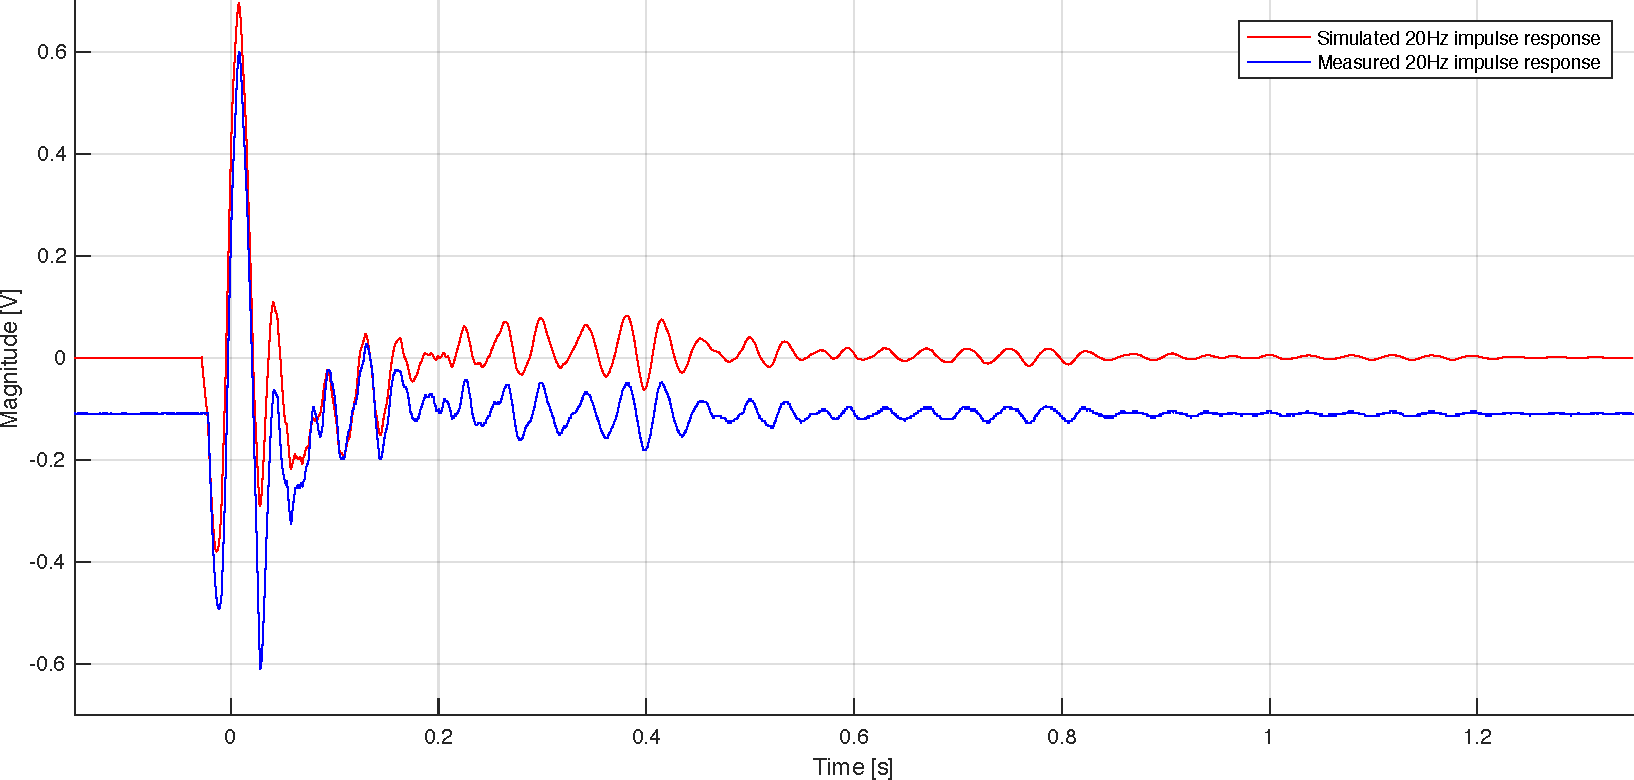
\includegraphics[width=\textwidth]{20Hz_impulse_response.pdf}
        \caption{Plot of the measured and simulated \gls{reverb} impulse response at \SI{20}{\hertz}.}
        \label{fig:tests:reverb:20Hz}
  \end{figure}
  
  \newpage
  
\subsubsection*{impulse response of \SI{50}{\hertz}}

\begin{figure}[htbp!]
    \centering
        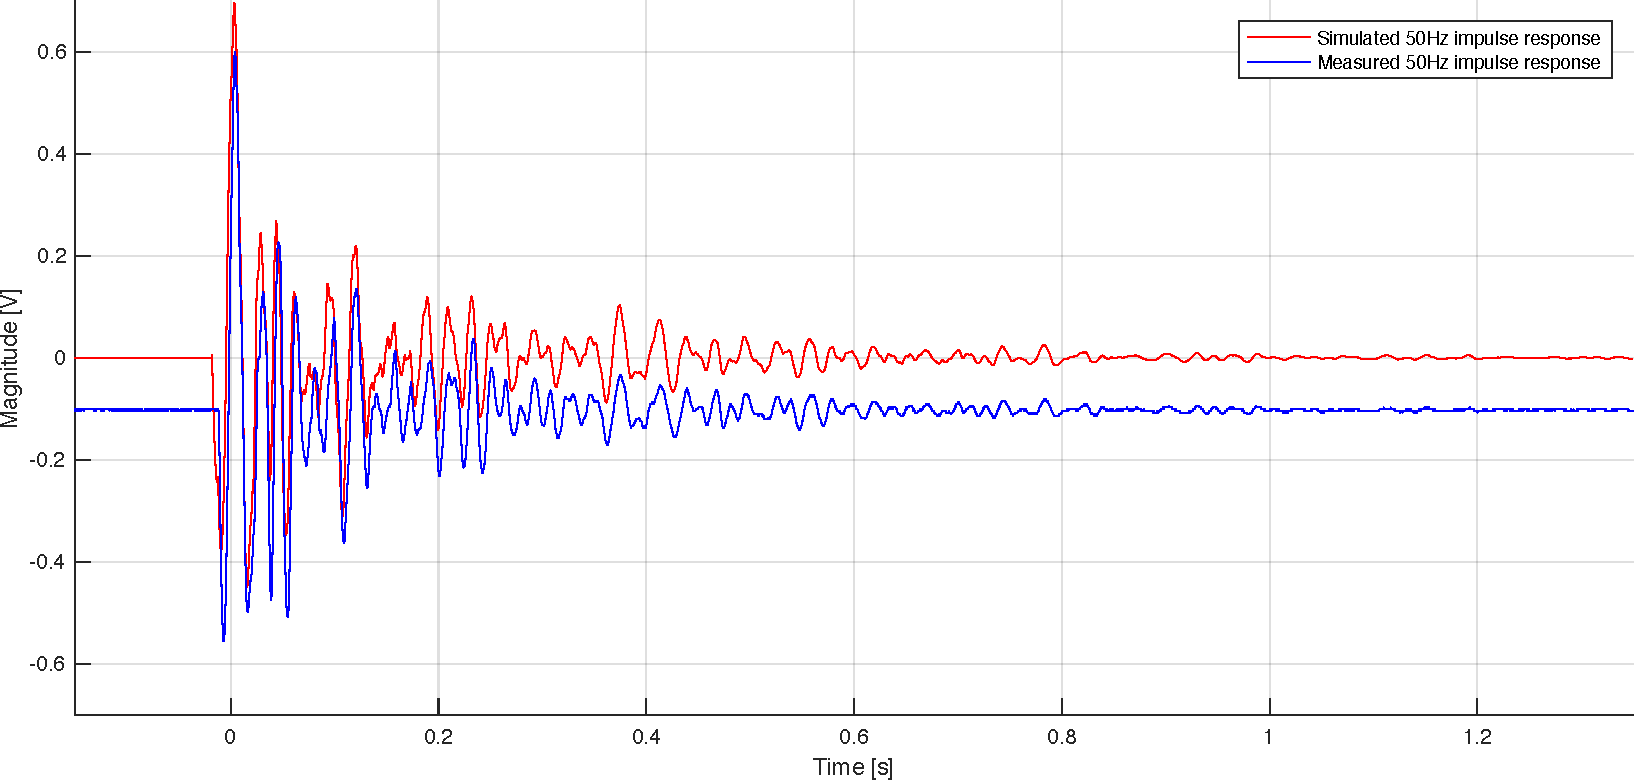
\includegraphics[width=\textwidth]{50Hz_impulse_response.pdf}
        \caption{Plot of the measured and simulated \gls{reverb} impulse response at \SI{50}{\hertz}.}
        \label{fig:tests:reverb:50Hz}
  \end{figure}

\subsubsection*{impulse response of \SI{200}{\hertz}}

\begin{figure}[htbp!]
    \centering
        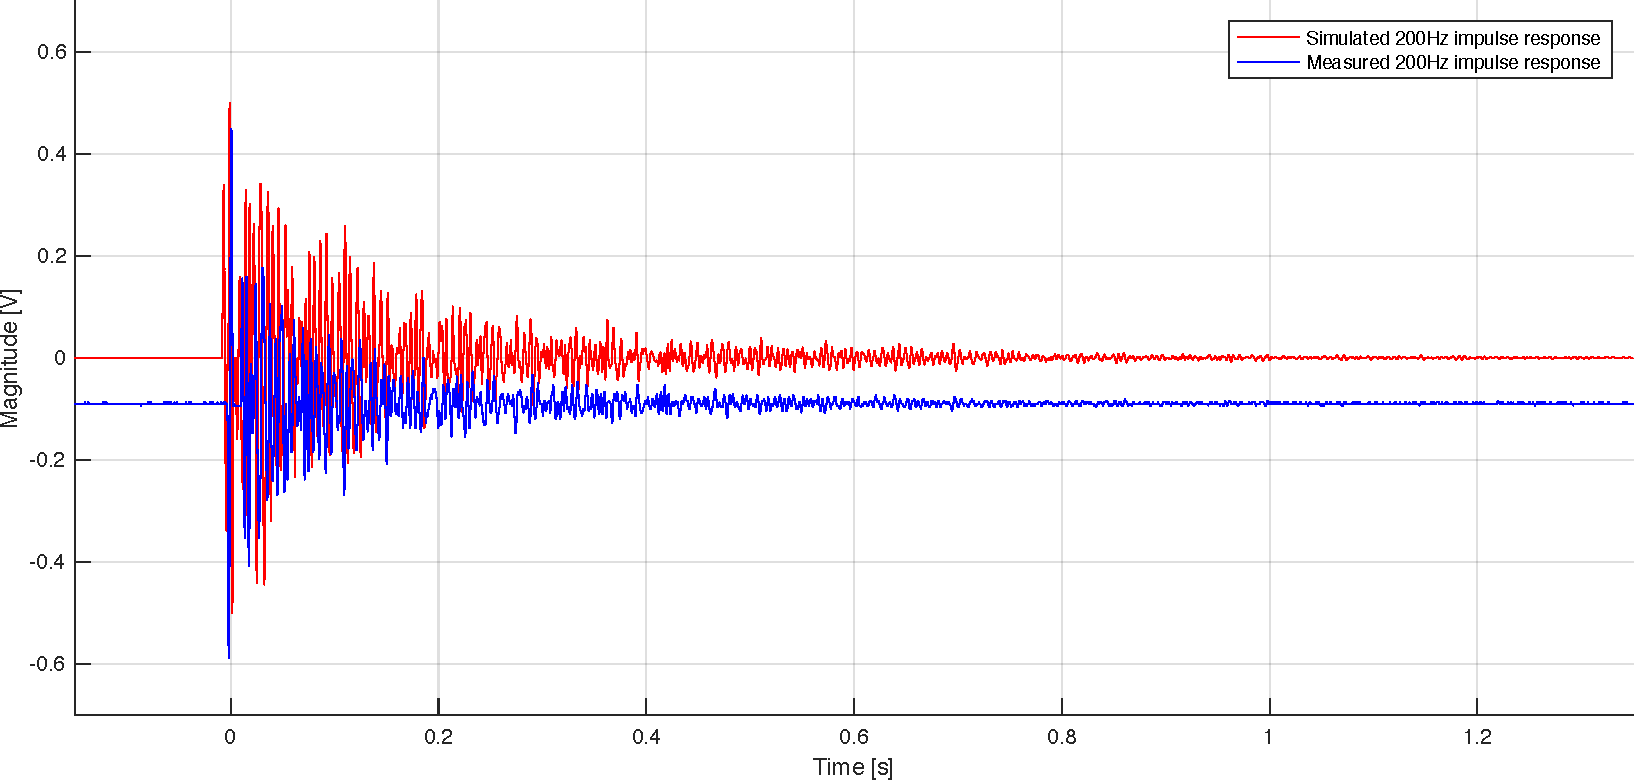
\includegraphics[width=\textwidth]{200Hz_impulse_response.pdf}
        \caption{Plot of the measured and simulated \gls{reverb} impulse response at \SI{200}{\hertz}.}
        \label{fig:tests:reverb:200Hz}
  \end{figure}

  \newpage
\subsubsection*{impulse response of \SI{1}{\kilo\hertz}}

\begin{figure}[htbp!]
    \centering
        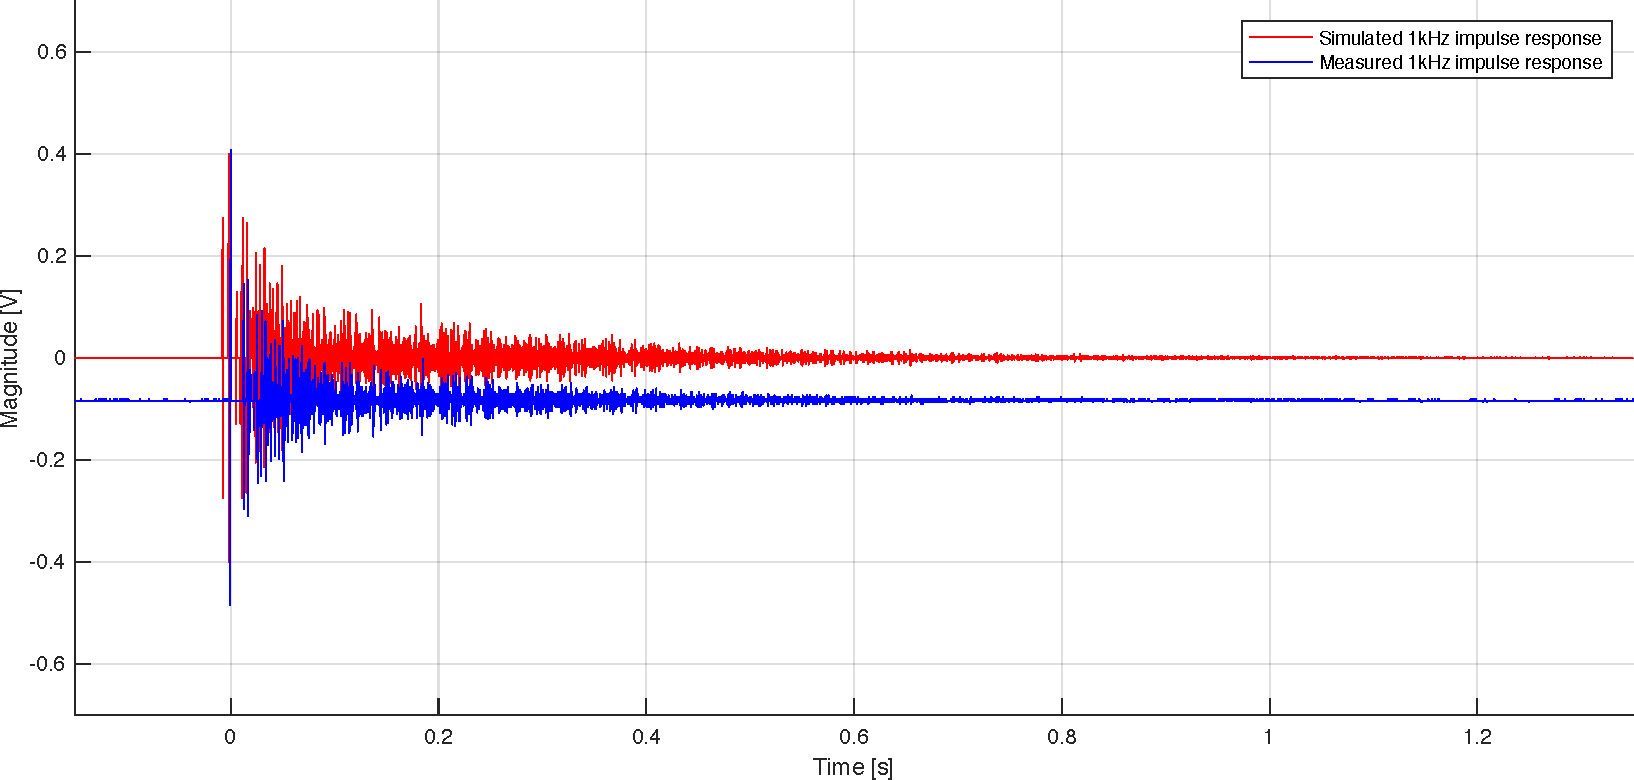
\includegraphics[width=\textwidth]{1kHz_impulse_response.pdf}
        \caption{Plot of the measured and simulated \gls{reverb} impulse response at \SI{1}{\kilo\hertz}.}
        \label{fig:tests:reverb:1kHz}
  \end{figure}
  
  
 \subsubsection*{impulse response of \SI{5}{\kilo\hertz}}

\begin{figure}[htbp!]
    \centering
        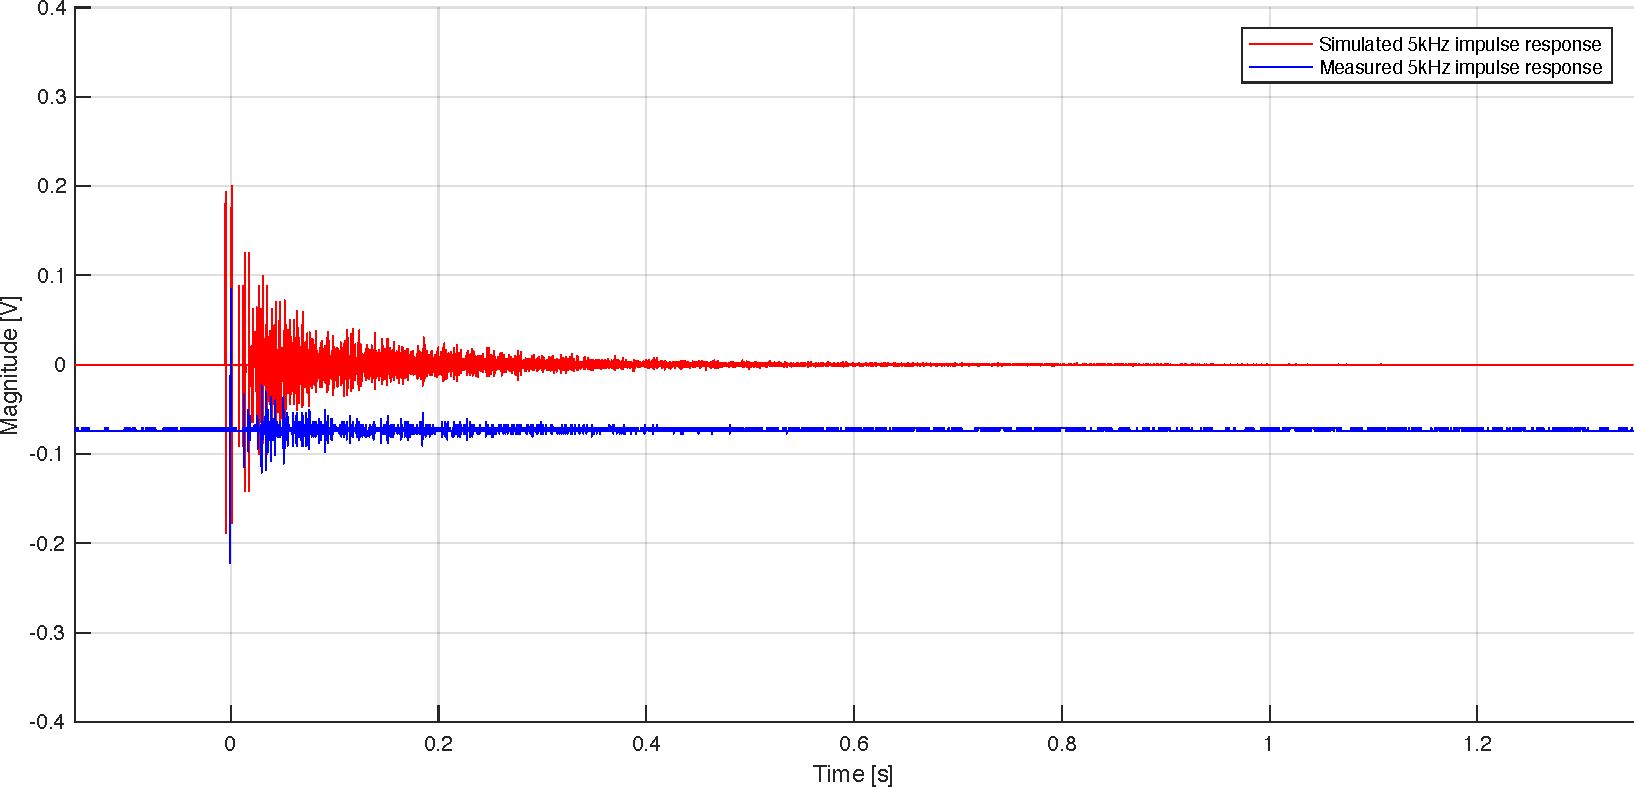
\includegraphics[width=\textwidth]{5kHz_impulse_response.pdf}
        \caption{Plot of the measured and simulated \gls{reverb} impulse response at \SI{5}{\kilo\hertz}.}
        \label{fig:tests:reverb:5kHz}
  \end{figure}
  
According to \autoref{sec:reverb_develop} the simulated data has more 1000 echo, and since the measured data are closely equal to the simulated data, \autoref{req:reverb1} is approved
  
  
\subsection{Test of requirement \autoref{req:reverb2}}
According to \autoref{fig:reverb_block_design} there is a gain called wet and dry, which is able to adjust the factor between the \gls{reverb} effect and the direct sound as following \autoref{eq:test:wetdry}

\begin{subequations}\label{eq:test:wetdry}
\begin{equation}
Dry = \text{user settings}
    \end{equation}
\begin{equation}
Wet = 1-\frac{\text{user settings}}{1} 
    \end{equation}
 \end{subequations}
    \startexplain
     \explain{$\text{user settings}$ is a user defined number between 0 and 1}{\si{1}}
    \stopexplain


Since the user interface not is implemented, \autoref{req:reverb2} is conditionally approved


\subsection{Test of requirement \autoref{req:reverb3}}
According to \autoref{eq:reverb_eq_f} and the following formulas in \autoref{sec:reverb_develop} the gain of every \gls{lpcf} can be changed, which will decrease or increase the number of echo from the six \gls{lpcf}. Since the number of echo can be changed, the \autoref{req:reverb2} is approved

\subsection{Test review of the Reverb Effect}
In this subsection, a short review will be shown of the \gls{reverb} effect test.

\begin{table}[H]
\centering
\caption{Recap of the requirements fulfillments for the chorus and flanger}
\label{test_of_reverb_table}
\begin{tabular}{|l|l|}
\hline
\rowcolor[HTML]{9B9B9B} 
\textbf{Requirement} & \textbf{Fulfillment State} \\ \hline
\textbf{\ref{req:reverb1}}    & \cmark                     \\ \hline
\textbf{\ref{req:reverb2}}    & \cmark*                     \\ \hline
\textbf{\ref{req:reverb3}}    & \cmark                     \\ \hline
\end{tabular}
\end{table}

    \startexplain
     \explain{\cmark  \hspace{4mm} is approved}{$\cdot$}
     \explain{\cmark* \hspace{1mm} is conditionally approved}{$\cdot$}
     \explain{\xmark \hspace{5mm} is not fulfilled}{$\cdot$}
    \stopexplain